\section{Die Garbage Collection}
\label{sec:shared_ptr}

Garbage Collection ist ein, im Zusammenhang mit dynamischen Sprachen,
weit verbreiteter Begriff, der
einen Mechanismus bezeichnet welcher für die Freigabe alloziierter
Ressourcen im laufenden Programm, zuständig
ist.

In \projectname{} wird diese mit Hilfe der, von Boost zur Verfügung
gestellten, !shared_ptr! Klasse umgesetzt.
Die Hauptimplementierung liegt hier in der Klasse
!lisp::environment! (Abschnitt \ref{sec:environment}),
die eine Hashtable mit allen
im Programm verwendeten Symbolen hält.
Symbole können auch nur über diese Klasse alloziiert werden.
Der Konstruktor der !symbol! Klasse wurde zu diesem Zweck als !private! deklariert.
Wenn nun ein Symbol über die !lisp::environment! Klasse angefordert wird,
so alloziiert diese Speicher für solch ein Symbol,
speichert einen Zeiger darauf in der verwalteten Hashtable
und umschließt es letztendlich mit einem !shared_ptr!
um diesen dann an den Aufrufer zurückzugeben.

Der Vorteil der genannten !shared_ptr! besteht nun darin,
dass diese einen Referenzzähler unterhalten,
der die Anzahl an Kopien, dieses Zeigers, im Speicher zählt.
Erreicht dieser Zähler den Wert $0$, so
wird die !lisp::environment! Klasse daüber informiert.
Selbige wägt dann ab ob das Symbol weiterhin benötigt
wird. Falls nicht wird es aus der gehaltenen Hashtable gelöscht.
Abbildung \ref{fig:garbage} veranschaulicht das Vorgehen.

%ich hoffe, das Bild stimmt einigermaßen…
\begin{figure}[htbp]
\centering
\captionabove{Speicherverwaltung}
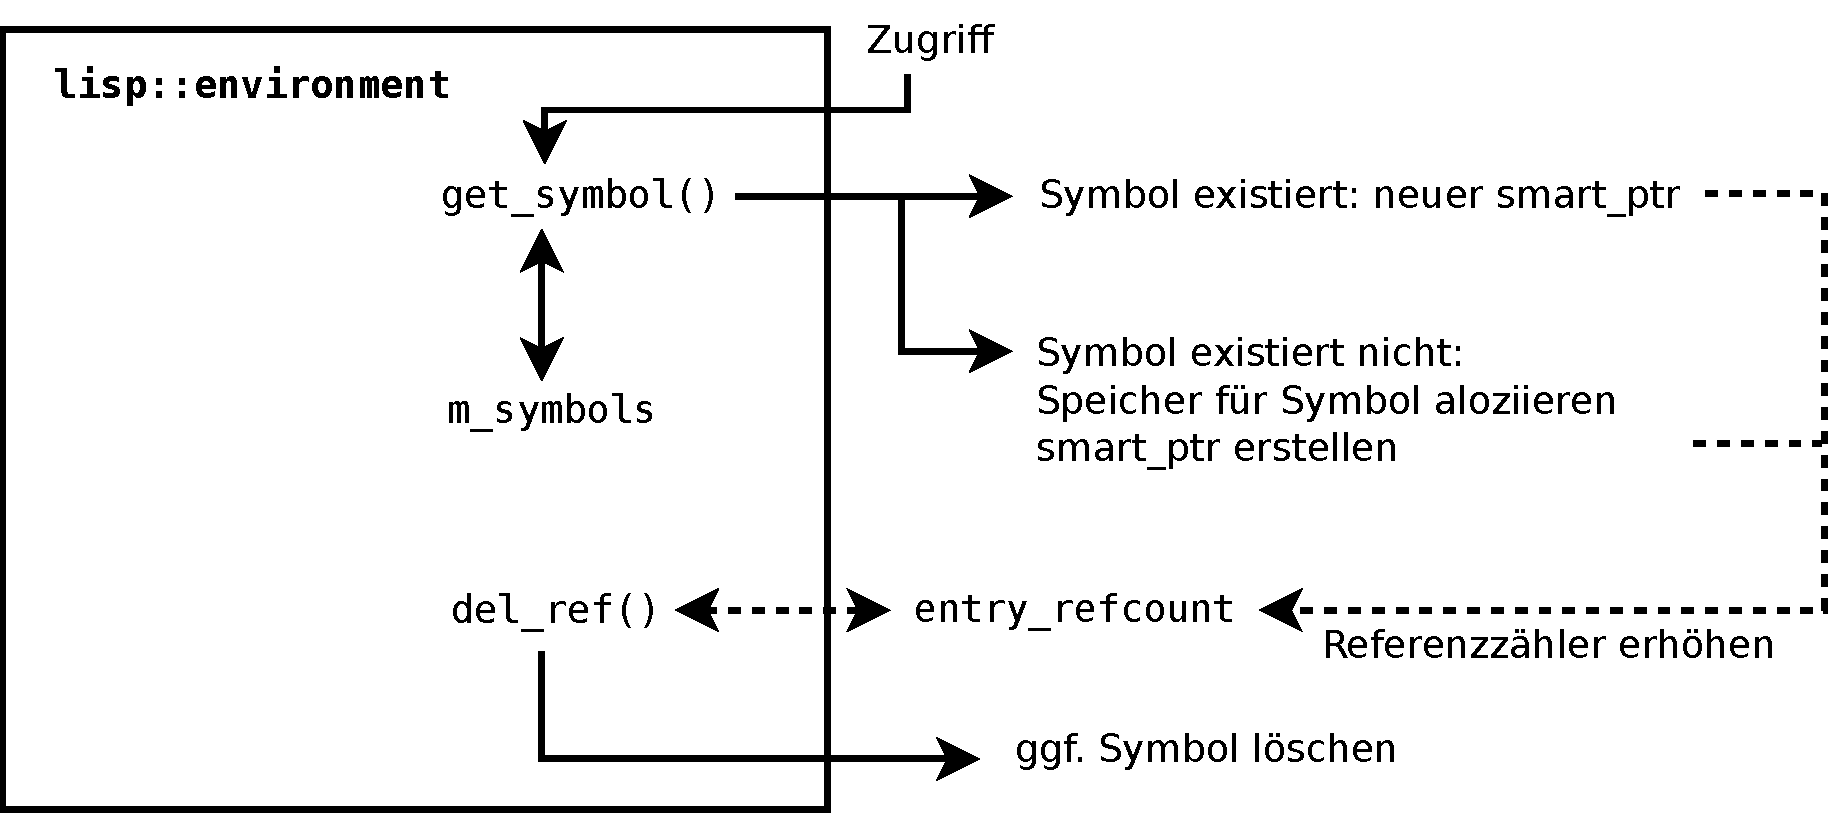
\includegraphics[width=0.8\textwidth]{images/garbage.pdf}
\label{fig:garbage}
\end{figure}

Hier ein Einzug aus der !lisp::environment! Klasse, der aufgerufen wird, wenn
ein Objekt ohne Referenzen im Speicher lebt:

\begin{lstlisting}[caption={Symbolbeseitigung}, label=lst:del_ref]
    void environment::del_ref(const std::string& name) 
    {
        symbol_table_t::iterator iter = m_symbols.find(name);

        if(iter == m_symbols.end())
            return;

        assert(entry_refcount(iter) > 0);

        --entry_refcount(iter);

        // Refcount is 0 -> Do garbage collection.
        if(entry_refcount(iter) <= 0 && entry_pointer(iter)->is_useless()) {
            delete entry_pointer(iter);

            m_symbols.erase(iter);
        }
    }
\end{lstlisting}


Für die Speicheralloziierung ist die Methode !get_symbol! zuständig:

\begin{lstlisting}[caption={Speicheralloziierung}, label=lst:get_symbol]
    symbol_ptr_t environment::get_symbol(const std::string& name)
    {
        symbol_table_t::iterator iter = m_symbols.find(name);
        symbol* sym_ptr = 0;

        if(iter == m_symbols.end()) {
            if(m_parent) {
                // Check parent.

                symbol_ptr_t sym = m_parent->get_symbol(name);

                if(sym)
                    return sym;
            }

            // Allocate memory for a new symbol.
            sym_ptr = new symbol(this, name);

            symbol_entry_t sym_entry(sym_ptr, 1);

            m_symbols.insert(m_symbols.begin(),
                             std::pair<std::string, symbol_entry_t>(name, sym_entry));
        }
        else {
            // Increase ref_count.
            ++entry_refcount(iter);

            sym_ptr = entry_pointer(iter);
        }

        symbol_ptr_t new_sym = symbol_ptr_t(sym_ptr, deleter());

        return new_sym;
    }
\end{lstlisting}
